\documentclass[a4paper,14pt]{article}
\usepackage{graphicx}
\usepackage{booktabs}
\usepackage[margin=1in]{geometry}
\usepackage{amsmath}
\usepackage[labelfont=bf]{caption}

\usepackage{hyperref}
\usepackage{subcaption}
\usepackage{listings} 
\usepackage{setspace}  
\usepackage{color}
\usepackage{xcolor}
\usepackage{listings}
\usepackage{xepersian}

\settextfont{XB Yas}
\setlength\parindent{0pt}


\begin{document}
	\fontsize{14}{14}\selectfont
	
	
	
	\begin{titlepage}
		\begin{center}
			
			\Huge
			
			\textbf{پروژه Bonus درس ارزیابی کارایی سیستم های کامپیوتری}
			
			\vspace{1cm}
			
			\LARGE
			
			
			نام استاد: دکتر احمد خونساری\\
				تاریخ: \today
			
			\vspace{1cm}
			
			
\includegraphics[width=0.5\textwidth]{teh.png}
			
			
			
			نویسندگان:\\
			
			\vspace{0.5cm}
			
			امیرحسین مهرورز: 810100484\\
			آرمان داوری: 810199153\\
			مجتبی مژگان فر: 810100471\\
			دانیال خلج: 810100515\\
			نیما شکری: 810199200\\
			یگانه کردی: 810100551\\
			محمدجواد دیانت: 810100348\\
			هادی قوامی نژاد: 810100438\\
			مینا فریدی: 810100430\\
			فاروق شایسته رودی: 810199198\\
			محمدمهدی یادگاری فرد: 81099308
			
			\vspace{0.5cm}
			
		
		
			
		\end{center}
	\end{titlepage}
	
	\newpage
	
	
	\textbf{مقدمه:}\\
	
	در این پروژه تمرین های فصل دوم و سوم کتاب Introduction-to-Probability به وسیله ی زبان پایتون حل شده است. با اجرای فایل simulation\_project\_group\_1.py برنامه ی اصلی شروع به کار کردن میکند و با پارامتر های مناسب میتوان شماره ی فصل و شماره ی هر سوال را وارد کرد تا خروجی جواب آن سوال به نمایش در بیاید.\\
	
	\textbf{کتابخانه های استفاده شده:}\\
	
	در طول برنامه نویسی این تمارین، کتابخانه های متعددی مورد استفاده قرار گرفته است که در زیر نام آنهارا بیان میکنیم:\\
	
	
	\begin{latin}
		matplotlib\\
		numpy\\
		gmpy2\\
		scipy\\
	\end{latin}

همچنین برخی از کتابخانه های خود پایتون نیز مورد استفاده واقع شد:\\

	\begin{latin}
		math\\
		random\\
		time\\
	\end{latin}
	
	
	\textbf{کد اصلی برنامه:}\\
	
	کد زیر مربوط به قسمت اصلی برنامه میباشد که کار مدیریت کل تمارین را بر عهده دارد. قبل از اجرای کد های حل تمرین ها، این کد اجرا میشود:\\
	
\fontsize{11}{11}\selectfont

\begin{latin}
	\begin{lstlisting}

if __name__ == '__main__':

  while True:
  chapter_number = int(input('Enter Chapter (2 or 3):'))

  if chapter_number not in [2,3]:
    print('Please enter a valid chapter (2 or 3)')
  else:
    if chapter_number == 2:
      while True:
        question_number = int(input('Enter Question (1,5,9,13,17,21,25,41):'))
        if question_number not in [1,5,9,13,17,21,25,41]:
          print('Please enter a valid question')
        else:
          if question_number == 1:
            solving_chapter2_problem_c2_q1()
          elif question_number == 5:
             solving_chapter2_problem_c2_q5()
          elif question_number == 9:
             solving_chapter2_problem_c2_q9()
          elif question_number == 13:
             solving_chapter2_problem_c2_q13()
          elif question_number == 17:
             solving_chapter2_problem_c2_q17()
          elif question_number == 21:
             solving_chapter2_problem_c2_q21()
          elif question_number == 25:
             solving_chapter2_problem_c2_q25()
          elif question_number == 41:
             solving_chapter2_problem_c2_q41()
          break

    elif chapter_number == 3:
      while True:
        question_number = int(input('Enter Question (1,5,13,21):'))
        if question_number not in [1,5,13,21]:
          print('Please enter a valid question')
        else:
          if question_number == 1:
            solving_chapter2_problem_c3_q1()
          elif question_number == 5:
            solving_chapter2_problem_c3_q5()
          elif question_number == 13:
            solving_chapter2_problem_c3_q13()
          elif question_number == 21:
            solving_chapter2_problem_c3_q21()
          break
    resume = input('Do you want to continue ? 
      (1 for yes and anything else for no):')
    if resume == '1':
      print('\n\n')
      continue
    else:
      break

	\end{lstlisting}
\end{latin}
	\fontsize{14}{14}\selectfont
	
	\textbf{کد های تمرین ها:}\\
	
	در این قسمت از گزارش، کد های مربوط به هر تمرین و توضیحات مربوط به آن کد قرار خواهد گرفت.\\
	
	\begin{center}
		{\LARGE
			\textbf{فصل دوم}
		}
	\end{center}

	\textbf{جواب سوال اول:}\\
	
	\fontsize{11}{11}\selectfont
	\begin{latin}
		\begin{lstlisting}
def calculate_pmf_of_2_games(nl_first,l_first,nl_second,
  l_second,p_tie,p_win):
  result = [0 for i in range(5)]
  # x -> 0 : losing , losing
  result[0] = l_first * l_second 
  # x -> 1 : not losing -> tie , losing + losing + not tising -> tie
  result[1] = (nl_first * p_tie * l_second) + (l_first * nl_second * p_tie)
  # x -> 2 : not losing -> tie , not losing -> tie + losing , not losing ->
    win + not losing -> win , losing
  result[2] = round((nl_first * p_tie * nl_second * p_tie) +
    (nl_first * p_win * l_second) + (l_first * nl_second * p_win),2)
  # x -> 3 : not losing -> win , not losing -> tie + not losing -> 
    tie , not losing -> win
  result[3] = round((nl_first * p_win * nl_second * p_tie) * 2,2)
  # x -> 4 : not losing -> win , not losing -> win
  result[4] = round(nl_first * p_win * nl_second * p_win,2)
  return result

def display_pmf(input_array):
  # displaying the probability of each item in the input
  for i in range(len(input_array)):
    print(f'P(x = {i}) : {input_array[i]}')
  # displaying otherwise probability 
  print(f'P(X > {len(input_array)}) : 0')


def solving_chapter2_problem_c2_q1():
  # probabilities:
  nl_first  = 0.4 # not losing in the first game probability
  nl_second = 0.7 # not losing in the second game probability
  l_first   = 0.6 # losing in the first game probability 
  l_second  = 0.3 # losing in the second game probability 

  p_tie     = 0.5 # probability of tie
  p_win     = 0.5 # probability of win

  # calling the caculte pmf with our probability definition
  result = calculate_pmf_of_2_games(nl_first,
    l_first,nl_second,l_second,p_tie,p_win)
  display_pmf(result)
		\end{lstlisting}
	\end{latin}
		\fontsize{14}{14}\selectfont
	
	در این سوال 2 بازی مطرح شده است که احتمال باختن، بردن و مساوی کردن را در هر دو بازی به ما داده است و برای هر پیشامد یک امتیازی در نظر گرفته است. این سوال از ما PMF این 2 بازی را میخواهد. برای بدست آوردن جواب این سوال میبایست تمامی حالت هارا در نظر بگیریم و تمامی احتمالات ممکن را بر اساس پیشامد ها بدست بیاوریم.\\
	
	خروجی این کد که در واقع نمایانگر PMF است به صورت زیر میباشد:
	

	\fontsize{11}{11}\selectfont
\begin{latin}
	\begin{lstlisting}
	
P(x = 0) : 0.18
P(x = 1) : 0.27
P(x = 2) : 0.34
P(x = 3) : 0.14
P(x = 4) : 0.07
P(X > 5) : 0

	\end{lstlisting}
\end{latin}
\fontsize{14}{14}\selectfont
	

\textbf{جواب سوال پنجم:}\\

\fontsize{11}{11}\selectfont
\begin{latin}
	\begin{lstlisting}

b = 30
c = 10
l = 15 # lambda = 15

def fact(n):
  fact = 1
  for i in range(1,n+1):
    fact = fact * i
  return fact

def poisson(k):
  return exp(-1 * l) * ((l**k)/fact(k))

def x_pmf(k):
  return poisson(k)

def y_pmf(k):
  if k == 0:
    prob = []
    for i in range (0,c):
    prob.append(poisson(i))
    return sum(prob)

  if k == (b-c):
    return x_pmf(b)  
 
  return poisson(k+c)

def discard(max_number):
  prob = []
  for i in range (0,max_number):
    prob.append(poisson(i))
  return 1 - sum(prob)

def solving_chapter2_problem_c2_q5():
  x = []
  for i in range(0,30):
    x.append(x_pmf(i))

  y = []
  for i in range(0,30):
    y.append(y_pmf(i))

  d = []
  for i in range(0,30):
    d.append(discard(i))

  plt.plot(range(0,30),x)
  plt.xlabel("Number of packets stored at the end of the first slot")
  plt.ylabel("PMF")
  plt.show()

  plt.plot(range(0,30),y)
  plt.xlabel("Number of packets stored at the end of the second slot")
  plt.ylabel("PMF")
  plt.show()

  plt.plot(range(0,30),d)
  plt.xlabel("Maximum number of packets that can be stored")
  plt.ylabel("Probability that some packets get discarded")
  plt.show()

	\end{lstlisting}
\end{latin}
\fontsize{14}{14}\selectfont

براي محاسبه تعداد پكت هايي كه در دو اسلات مي آيند سوال پارامتري است. چيزي كه مي توانيم نشان دهيم شكل خروجي با
استفاده از پارامترهايي است كه بدست مي آيد.
لذا نمودار تعداد پكت هاي اسلات اول و تعداد پكت هاي اسلات دوم رسم شده است. نمودارها بيانگر تاثير تغيير پارامترها مي
باشد.\\

خروجی این سوال به صورت زیر میباشد:\\

\begin{center}
	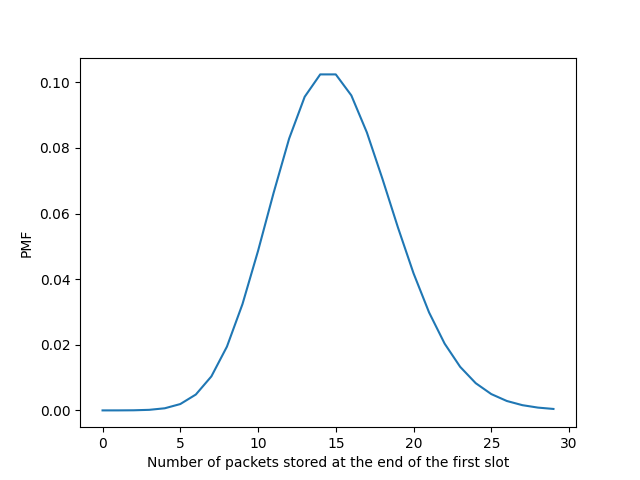
\includegraphics[width=1\textwidth]{pic1.png}
\end{center}
\begin{center}
	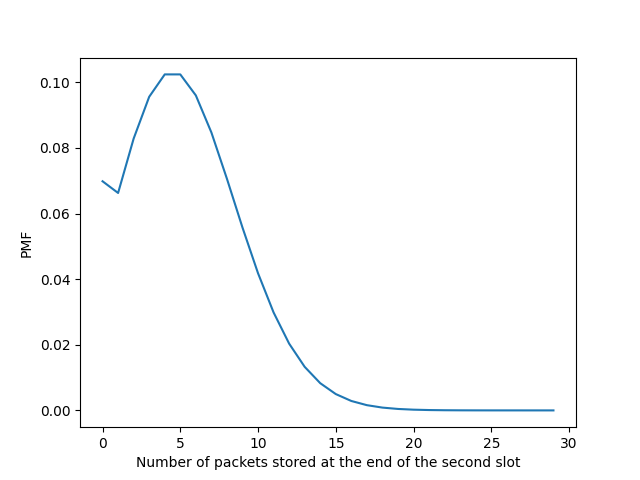
\includegraphics[width=1\textwidth]{pic2.png}
\end{center}
\begin{center}
	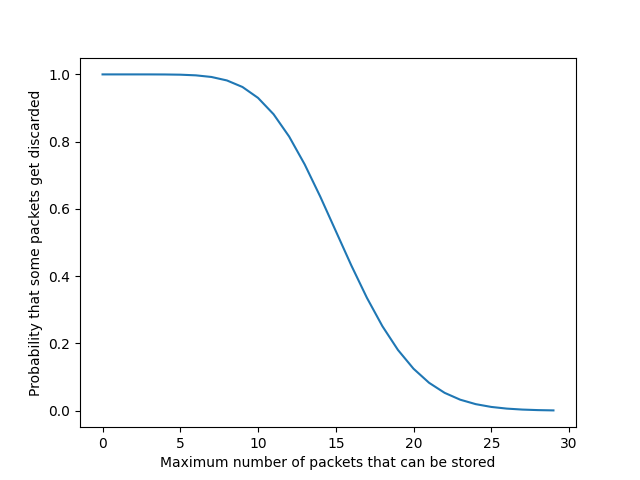
\includegraphics[width=1\textwidth]{pic3.png}
\end{center}

\textbf{جواب سوال نهم:}

\fontsize{11}{11}\selectfont

\begin{latin}
	\begin{lstlisting}

n = 99
p = 0.4
k = np.linspace(10,60,num=50,endpoint=False)
ans = []


def facto (n):
  fact = 1
  for i in range(1,n+1):
    fact = fact * i

  return fact

def combo(n, k):
  temp1 = facto(n)
  temp2 = facto(k)
  temp3 = facto(n-k)
  cmb = temp1/(temp2*temp3)
  return cmb

def q9(n,k,p):
  temp1 = combo(n,k)*pow(p,k)*pow(1-p,n-k)
  temp2 = combo(n,k-1)*pow(p,k-1)*pow(1-p,n-k+1)
  return temp1/temp2

def solving_chapter2_problem_c2_q9():
  print(k)

  for ks in k:
    ans.append(q9(n,int(ks),p))

  plt.plot(ans,k)
  plt.hlines(y = (n+1)*p, xmin = 0, xmax = 6, color ='r', linestyle='--')
  plt.vlines(x = 1, ymin=0, ymax = 60, color = 'y', linestyle = '--')
  plt.text(0, ((n+1)*p)+0.5, '(n+1)*p', ha ='left', va ='bottom')
  plt.text(1, 0.8, 'Ratio = 1',rotation ='vertical', ha ='right', va ='bottom')
  plt.xlabel("Ratio calculated with different values of K")
  plt.ylabel("values of K")

  plt.show()

	\end{lstlisting}
\end{latin}
	\fontsize{14}{14}\selectfont
	
	
	در ابتدا به ازای مقادیر صفر تا $n$ نسبتی که از طریق تقسیم $ p_x(k) $ به $ p_x(k-1) $ بدست می آید را محاسبه می کنیم. مشاهداتی که به شکل گرافیکی در نمودار آورده شده نشان می دهد به ازای $k$ کوچکتر مساوی $k^*$ مقدار $k-kp$ کوچکتر مساوی $ (n+1)p-kp $ می شود.
	
	\noindent در نتیجه همانطور که در نمودار ترسیم شده مشهود است نسبت محاسبه شده فوق بزرگتر و یا مساوی 1 می شود که نشان می دهد احتمال اکیدا غیرنزولی است و در صورتی که $k$ بزرگتر از $k^*$ باشد، این نسبت محاسبه شده با توجه به نمودار مقداری کمتر از 1 خواهد داشت که تابع احتمال نیز اکیدا نزولی خواهد بود.\\
	
	نتیجه ی این کد به صورت زیر میباشد:\\
	
	
	
	
\begin{latin}
	\begin{lstlisting}
[10. 11. 12. 13. 14. 15. 16. 17. 18. 19.
 20. 21. 22. 23. 24. 25. 26. 27. 28. 29.
 30. 31. 32. 33. 34. 35. 36. 37. 38. 39.
 40. 41. 42. 43. 44. 45. 46. 47. 48. 49.
 50. 51. 52. 53. 54. 55. 56. 57. 58. 59.]
	\end{lstlisting}
\end{latin}

همچنین نمودار حاصل از اجرای این کد به صورت زیر رسم میشود:\\

\begin{center}
	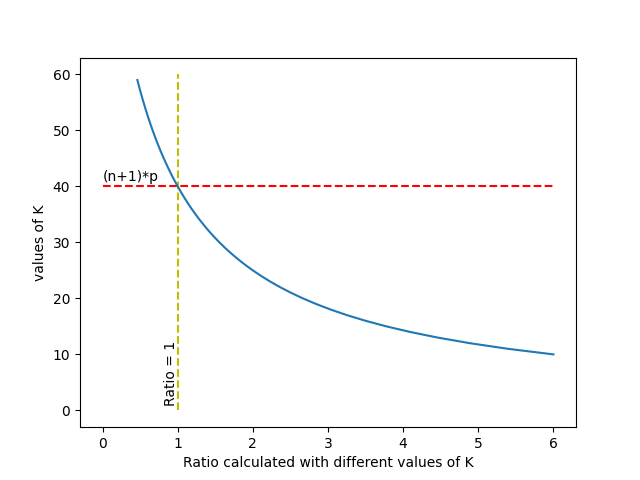
\includegraphics[width=1\textwidth]{pic4.png}
\end{center}

\textbf{جواب سوال سیزدهم:}\\


\fontsize{11}{11}\selectfont

\begin{latin}
	\begin{lstlisting}
		
def pmf_girls (g, naturals, adoptedgirls):
  all = naturals + adoptedgirls
  if (adoptedgirls>g or all <g):
    return (0)
  else:
    return math.comb(naturals,g-2) * math.pow(0.5,naturals)

def solving_chapter2_problem_c2_q13():
  # print("insert number of the girls to find PMF")
  # g = int(input()) #pmf variable (num of girls)
  g = 3 #for example

  naturals = 5  # number of natural children
  adoptedgirls = 2  # number of adopted girls

  print(pmf_girls (g, naturals, adoptedgirls))
		
	\end{lstlisting}
\end{latin}
\fontsize{14}{14}\selectfont 


در این سوال \lr{pmf} تعداد دخترهای خانواده خواسته شده است. این خانواده 5 فرزند طبیعی دارد که جنسیت شان را نمی دانیم همچنین 2 دختر دارد که به سرپرستی گرفته شده اند.

به عنوان مثال میخواهیم بدانیم احتمال اینکه تعداد کل دخترها 3 باشد چقدر است. در تابع تعریف شده ابتدا $g$ مورد تقاضا را بررسی می کنیم که در بازه مورد نظر باشد. $g$ بایستی حداقل 2 باشد و حداکثر نیز بایستی از تعداد کل بچه ها بیشتر باشد در غیراینصورت مقدارش 0 می شود. انتخاب $g-2$ از فرزندان طبیعی را محاسبه می کنیم و $return$ می کنیم.\\

خروجی این کد به صورت زیر است:\\
\begin{latin}
0.15625
\end{latin}
	
	\textbf{جواب سوال هفدهم:}\\
	
	\fontsize{11}{11}\selectfont
	
	\begin{latin}
		\begin{lstlisting}
			
def cel_to_fahr(cel_mu: float, cel_sigma: float) -> float:
  """
  since we know transform is linear, we can use the inverse transform
  fahr  = (cel * 9 / 5) + 32

  and new mean and sigma are:

  E[fahr] = (E[cel] * 9 / 5) + 32;

  var(fahr) = (9/5)^2 * var(cel)
  => sigma(fahr) = (9/5) * sigma(cel)

  """
  fahr_mu    = cel_mu * 9 / 5 + 32
  fahr_sigma = cel_sigma * 9 / 5

  return fahr_mu, fahr_sigma

def normal_pdf(x, mu:float, sigma:float) -> float:
  """
  normal distribution pdf function
  """
  return (1.0 / np.sqrt(2 * np.pi * sigma ** 2)) *
  np.exp(-0.5 * (x - mu) ** 2 / sigma ** 2)

def make_plot(axs, title: str, mu: float, sigma: float) -> None:
  """
  axs: matplotlib axes
  title: string
  mu: float
  sigma: float
  ------------------------
  We want to plot the distribution of the temperature
  and since we know it is normal, we can use the normal distribution function
  from scipy.stats.norm to plot it.
  for range of x, we use mu-3*sigma to mu+3*sigma
  to make sure we get a full range of the distribution.

  The normal range includes the Mu + - Sigma range, so we separate this area.
  """
  x     = np.linspace(mu - 3 * sigma, mu + 3 * sigma, 100)
  y     = normal_pdf(x, mu, sigma)
  left  = mu - sigma
  right = mu + sigma

  axs.plot(x, y, "k")
  axs.set_title(title, fontsize=14, loc="left")
  axs.vlines(left, 0,
  normal_pdf(left, mu, sigma),
  colors="r", linestyles="dashed")
  axs.text(
  left + (0.5 if left == 0 else 2),
  normal_pdf(left, mu, sigma) / 2,
  int(left),
  fontsize=10, 
  )
  axs.vlines(right, 0,
  normal_pdf(right, mu, sigma),
  colors="r", linestyles="dashed")
  axs.text(
  right - (5 if right % 10 == 0 else 9),
  normal_pdf(right, mu, sigma) / 2,
  int(right),
  fontsize=10,
  )
  axs.spines["top"  ].set_visible(False)
  axs.spines["right"].set_visible(False)
  axs.spines["left" ].set_visible(False)
  axs.tick_params(left=False, labelleft=False)


def solving_chapter2_problem_c2_q17():
  fig, axs = plt.subplots(1, 2, figsize=(10, 6))

  celsius_mu    = 10
  celsius_sigma = 10

  fahrenheit_mu, fahrenheit_sigma = cel_to_fahr(celsius_mu, celsius_sigma)

  make_plot(
  axs[0], r"$\mathbf{Temperature \; in}$" +"\nCelsius",
  celsius_mu,
  celsius_sigma
  )
  make_plot(
  axs[1],
  r"$\mathbf{Temperature \; in}$" + "\nFahrenheit",
  fahrenheit_mu,
  fahrenheit_sigma,
  )
  plt.show()
			
		\end{lstlisting}
	\end{latin}
	\fontsize{14}{14}\selectfont 
	

این کد شامل سه فانکشن عملیاتی به صورت زیر است:
\begin{itemize}
	\item \lr{Cel\_to fahr}
	\subitem 	این فانکشن با توجه به فرمول تبدیل سلسیوس به فارنهایت $\mu$  و $\sigma$ مربوط به تابع توزیع فارنهایت را محاسبه می کند.
	\item \lr{Normal\_pdf}
	\subitem	محاسبه تابع توزیع نرمال با استفاده از ورودی های لازم
	\subitem \lr{X,$\mu$,$\sigma$}
	\item \lr{Make\_plot}
	\subitem	برای رسم توزیع  دما استفاده می شود
	\subitem	از آنجایی که می دانیم تابع توزیع نرمال است، می توانیم از تابع \lr{Normal\_pdf} برای رسم آن استفاده کنیم. برای محدوده \lr{x}، ما از $\mu - 3 * \sigma$ تا $\mu + * \sigma$ استفاده می کنیم تا مطمئن شویم که طیف کاملی از توزیع را دریافت می کنیم.
	\subitem	محدوده نرمال شامل محدوده $\mu \mp \sigma$ می شود، بنابراین این ناحیه را نیز به صورت مشخص جدا می کنیم.
\end{itemize}
	
	نتیجه ی خروجی این کد به صورت زیر است:\\
	
	\begin{center}
		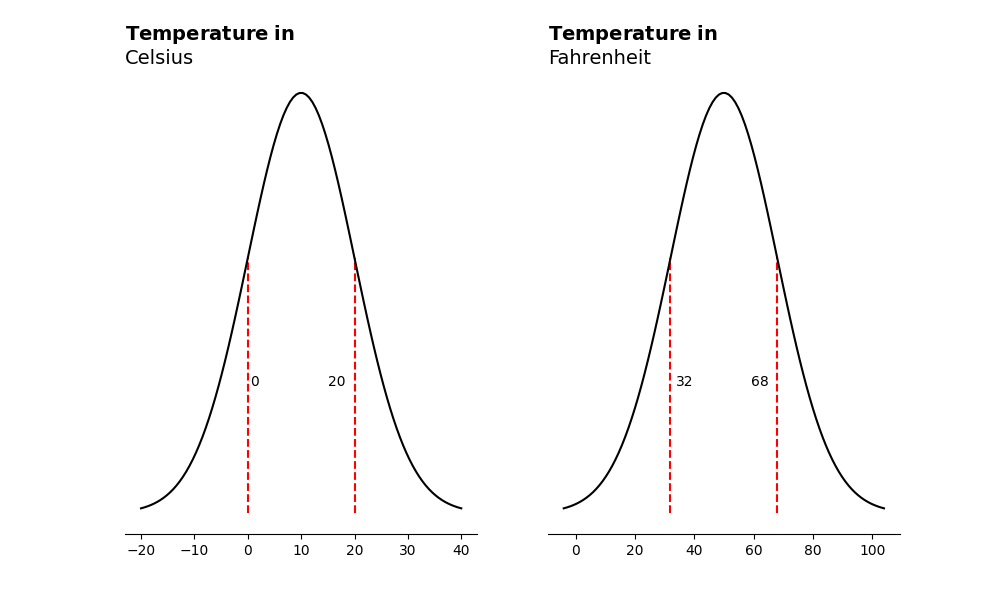
\includegraphics[width=1\textwidth]{pic5.png}
	\end{center}
	
	\textbf{جواب سوال بیست و یکم}\\
	
		\fontsize{11}{11}\selectfont
	
	\begin{latin}
		\begin{lstlisting}
			
def tossCoin():
  resualt=None
  if random.randint(0,1)==0:
    resualt='head'
  else:
    resualt='tail'
  return resualt


# Press the green button in the gutter to run the script.

def solving_chapter2_problem_c2_q21():
  deposit = 0
  while True:
    numberOfTosses=0
    result=tossCoin()
    while result=='head':
      numberOfTosses+=1
      result=tossCoin()
      if numberOfTosses>0:
        deposit += pow(2, numberOfTosses)
        print('Congrats!! You have earned ' + str(pow(2, numberOfTosses)) +
          '$ In this round!')
      else:
        print('Sorry :( You did not win in this round')

      print('Total Deposit: '+str(deposit)+'$ ')
      print()
      print('------------------------------------------------')
      print()
      time.sleep(1.5)
			
		\end{lstlisting}
	\end{latin}
	\fontsize{14}{14}\selectfont 
	
	
	
	در این سوال سکه ای را پرتاب می کنیم اگر شیر بیاید می شماریم. مادامی که شیر بیاید می شماریم و هنگامی که خط آمد، 2 به توان آن مقدار پول می دهد.
	
	\noindent قطعه کد ما شبیه سازی پرتاب سکه است. مکرراً سکه را می اندازد و وابسته به اینکه چه تعدادی شیر آمده اعلام می کند در آن راند چقدر پیروز شده ایم.
	
	\noindent نشان داده می شود که به سمت بی نهایت رشد پیدا می کند.\\
	
	با توجه به شانسی بودن احتمال شیر یا خط، نتیجه ی خروجی متفاوت است. در اینجا چند بار آزمایش را نمایش میدهیم:\\
	
		\begin{latin}
		\begin{lstlisting}
			
Congrats!! You have earned 2$ In this round!
Total Deposit: 2$

-------------------------------------------------

Congrats!! You have earned 2$ In this round!
Total Deposit: 4$

-------------------------------------------------

Congrats!! You have earned 2$ In this round!
Total Deposit: 6$

-------------------------------------------------

Congrats!! You have earned 2$ In this round!
Total Deposit: 8$

-------------------------------------------------

Sorry :( You did not win in this round
Total Deposit: 8$

-------------------------------------------------

Sorry :( You did not win in this round
Total Deposit: 8$

-------------------------------------------------

Sorry :( You did not win in this round
Total Deposit: 8$

-------------------------------------------------

Sorry :( You did not win in this round
Total Deposit: 8$

-------------------------------------------------

Sorry :( You did not win in this round
Total Deposit: 8$

-------------------------------------------------

Congrats!! You have earned 2$ In this round!
Total Deposit: 10$

-------------------------------------------------

Congrats!! You have earned 4$ In this round!
Total Deposit: 6$

-------------------------------------------------

Sorry :( You did not win in this roundTotal Deposit: 6$

-------------------------------------------------
			
		\end{lstlisting}
	\end{latin}

\textbf{جواب سوال بیست و پنجم}\\


		\fontsize{11}{11}\selectfont

\begin{latin}
	\begin{lstlisting}
		
def M_i_randGenerator (m,M,n):
  for i in range(0,n):
    M[i] = rn.randint(0,m)

#M = [0,1,2]

def calculate_L(m,M,n,L):
  for x in range(0,n):
    for y in range(0,m):
      if y+1 <= M[x]:
        L[y] = L[y] + 1

def sigma_Mk(M,n):
  sum = 0
  for k in range (0 , n):
    sum = sum + M[k]
  return sum

def calculate_Joint_PMF (n,M,m,Prob_IJ,sum):
  for i in range(0,n):
    for j in range(0,m):
      if j+1 <= M[i] :
        Prob_IJ[i][j] = 1 / sum
      else:
        Prob_IJ[i][j] = 0.0
      print("Joint PMF of (", i+1 , "," , j+1 , ") is: " , Prob_IJ[i][j])


def calculate_Marginal_PMF_I (n , m,Prob_I,M,sum):
  for i in range(0,n):
    Prob_I[i] = M[i] / sum
    print( "Marginal PMF of I (", i+1 , ") is: ", Prob_I[i] )

def calculate_Marginal_PMF_J (n , m,L,Prob_J,sum):
  for j in range(0,m):
    Prob_J[j] = L[j] / sum
    print( "Marginal PMF of J (", j+1 , ") is: ", Prob_J[j] )

def probabilty_ij(n,m,p_ij):
  for i in range(0,n):
    for j in range(0,m):
      p_ij[i][j] = rn.random()
      print("probabilty of (",i+1, "," ,j+1,")" , p_ij[i][j])

def expected_value(n,M,p_ij,a,b):
  sigma = 0
  for i in range(0,n):
    for j in range(0,M[i]):
      sigma = sigma + ( p_ij[i][j] * a ) + ( (1 - p_ij[i][j]) * b )
  print("Exptected Value is: " , sigma)

def solving_chapter2_problem_c2_q25():

  n = int( input("enter integer value for n (4 in the question): " ) )
  m = int( input("enter integer value for m (3 in the question): ") )
  a = int( input("enter integer value for a (1 in the question): " ) )
  b = int( input("enter integer value for b (-1 in the question): " ) )
  print("-" * 60)

  """
  n=3
  m=4
  a = 1
  b = -1
  """

  M = [0] * n
  L = [0] * m
  sum = 0

  Prob_IJ = [[0]*m]*n
  Prob_I = [0] * n
  Prob_J = [0] * m
  p_ij = [[0]*m]*n

  M_i_randGenerator (m,M,n)
  print("M array is:" , M)
  print("-" * 60)

  calculate_L(m,M,n,L)
  print("L array is:" , L)
  print("-" * 60)

  sum = sigma_Mk(M,n)
  print("sum is:" , sum)
  print("-" * 60)

  calculate_Joint_PMF (n,M,m,Prob_IJ,sum)
  print("-" * 60)

  count = 0
  for i in range(0,n):
    for j in range(0,m):
      count = count + Prob_IJ[i][j]
  print("count is: ", count)
  print("-" * 60)

  calculate_Marginal_PMF_I (n , m,Prob_I,M,sum)
  print("-" * 60)

  calculate_Marginal_PMF_J (n , m,L,Prob_J,sum)
  print("-" * 60)

  probabilty_ij(n,m,p_ij)
  print("-" * 60)

  expected_value(n,M,p_ij,a,b)
  print("-" * 60)
		
	\end{lstlisting}
\end{latin}
\fontsize{14}{14}\selectfont 


در این سوال \lr{n} دانش آموز دریم و \lr{m} سوال. دانش آموز \lr{i} ام $m_i$ تا سوال اول را جواب می دهد و بقیه سوالات را جواب نداده است. پس به تعداد $m_i$ ها جواب داریم. \lr{joint pmf} آن 1 تقسیم بر سیگمای مخرج می باشد اگر \lr{j}	ها کمتر از $m_i$ ها باشد.

\noindent تابعی داریم که به صورت رندوم  $m_i$ ها را مشخص می کنیم. تابعی برای محاسبه سیگمای مخرج داریم. تابعی برای محاسبه اینکه چند نفر به سوال \lr{j} ام جواب داده اند را محاسبه می کند و در نهایت تابعی داریم که برای \lr{i} و \lr{j} تابع \lr{pmf} حاشیه ای را محاسبه می کند.

\noindent در قسمت ب، فرض می کنیم جواب تحویل داده شده با احتمال $p_{ij}$ درست است و با احتمال $ 1 - P_{ij} $ نادرست است. اگر درست باشد \lr{a} پوینت و اگر غلط باشد \lr{b} پوینت می گیرد در نهایت مقدار \lr{Expected Value} در تابع آن محاسبه می گردد.\\

خروجی این کد به ازای n=4 و m=3 و a=1 و b=-1 به صورت زیر میباشد:\\

\begin{latin}
	\begin{lstlisting}

---------------------------------------------
M array is: [0, 1, 2, 0]
---------------------------------------------
L array is: [2, 1, 0]
---------------------------------------------
sum is: 3
---------------------------------------------
Joint PMF of ( 1 , 1 ) is:  0.0
Joint PMF of ( 1 , 2 ) is:  0.0
Joint PMF of ( 1 , 3 ) is:  0.0
Joint PMF of ( 2 , 1 ) is:  0.3333333333333333
Joint PMF of ( 2 , 2 ) is:  0.0
Joint PMF of ( 2 , 3 ) is:  0.0
Joint PMF of ( 3 , 1 ) is:  0.3333333333333333
Joint PMF of ( 3 , 2 ) is:  0.3333333333333333
Joint PMF of ( 3 , 3 ) is:  0.0
Joint PMF of ( 4 , 1 ) is:  0.0
Joint PMF of ( 4 , 2 ) is:  0.0
Joint PMF of ( 4 , 3 ) is:  0.0
---------------------------------------------
count is:  0.0
---------------------------------------------
Marginal PMF of I ( 1 ) is:  0.0
Marginal PMF of I ( 2 ) is:  0.3333333333333333
Marginal PMF of I ( 3 ) is:  0.6666666666666666
Marginal PMF of I ( 4 ) is:  0.0
---------------------------------------------
Marginal PMF of J ( 1 ) is:  0.6666666666666666
Marginal PMF of J ( 2 ) is:  0.3333333333333333
Marginal PMF of J ( 3 ) is:  0.0
---------------------------------------------
probabilty of ( 1 , 1 ) 0.6086080476233853
probabilty of ( 1 , 2 ) 0.4557177120051581
probabilty of ( 1 , 3 ) 0.2898182856630127
probabilty of ( 2 , 1 ) 0.2515811634212529
probabilty of ( 2 , 2 ) 0.747979635611269
probabilty of ( 2 , 3 ) 0.37566283360759256
probabilty of ( 3 , 1 ) 0.00934753256118237
probabilty of ( 3 , 2 ) 0.8965086235710871
probabilty of ( 3 , 3 ) 0.26113698759359616
probabilty of ( 4 , 1 ) 0.7549944764423108
probabilty of ( 4 , 2 ) 0.06808941759715448
probabilty of ( 4 , 3 ) 0.767159373012873
---------------------------------------------
Exptected Value is:  0.15615674096355203
---------------------------------------------

	\end{lstlisting}
\end{latin}


\textbf{جواب سوال چهل و یکم:}\\

		\fontsize{11}{11}\selectfont
\begin{latin}
	\begin{lstlisting}

def solving_chapter2_problem_c2_q41():
  w = 50 # week
  d = 5 #day
  p = 0.02
  n = d * w
  k = 5
  lambdaa = n * p # for part b

  pay_t = [10,20,50] # Ticket prices for part c
  p_pay_t = [0.5,0.3,0.2] # respective probabilities for part c

  pk= comb(n,k) * p**k * (1-p)**(n-k)
  print("P(X = k) = " , pk)

  # defining list of r values
  r_values = list(range(16))
  # list of pmf values
  dist = [binom.pmf(r, n, p) for r in r_values ]
  # plotting the graph
  plt.bar(r_values, dist)
  plt.show()

  approximation = e**(-lambdaa) * (lambdaa ** k / fac(k))
  print("Poisson  approximation of part a : " , approximation)


  tp_pay_t = dot(p, p_pay_t)
  p_mean = sum(dot(pay_t,tp_pay_t))
  mean = n * p_mean
  p_var = sum(dot(power(pay_t,2),tp_pay_t)) - p_mean**2
  var = n * p_var

  print("mean: " , mean )
  print("Variance: " , var )


	\end{lstlisting}
\end{latin}
		\fontsize{14}{14}\selectfont
	

در پارت نخست آزمایش برنولی می باشد که از قطعه کد $pk= comb(n,k) * p**k * (1-p)**(n-k)$ استفاده می نماییم.
به جهت افزایش قدرت تغییر و انعطاف در برنامه، \lr{Expected Value} را محاسبه نکردیم بلکه می توان به ازای $k$ هر مقداری قرار داد و احتمال آن را محاسبه نمود.
در صورتی که \lr{Expected Value} را بخواهیم منطبق بر صورت سوال به $k$ مقدار 5 می دهیم و از لاندا که در پارت دوم استفاده شده است، می توانیم استفاده کنیم.
قسمتی اضافه تر از خواسته صورت سوال نیز انجام شده است که آن محاسبه $PMF$ است.

برای پارت دوم از \lr{Poisson Approximation} منطبق در ذیل استفاده می کنیم.

{
	\centering
	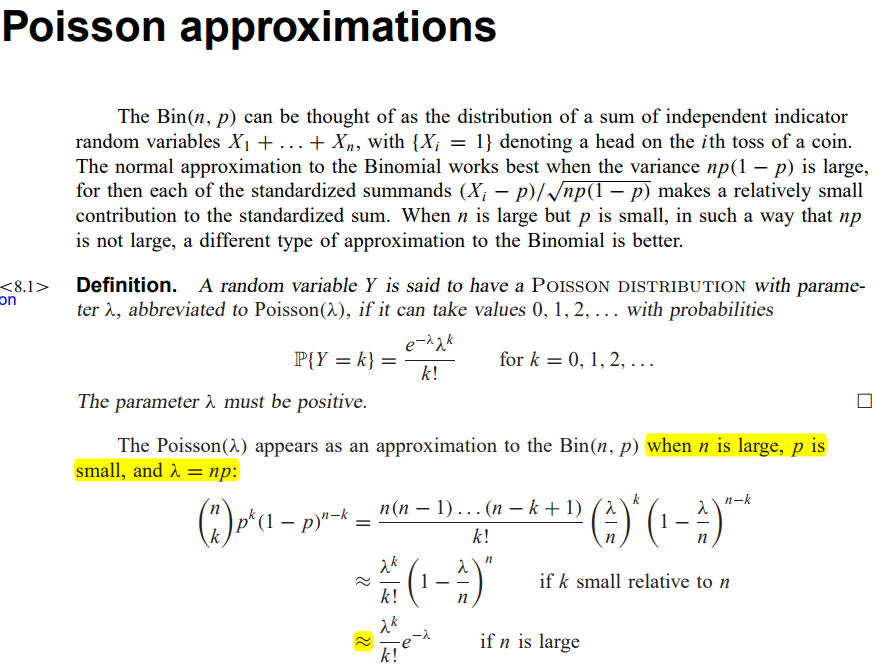
\includegraphics[width=0.7\textheight]{approximations.png}
	
}

در پارت سوم قیمت برای بلیط ها تغیین شده است و درصد داده شده است. قیمت بلیط ها در \lr{pay\_t} و احتمال متناسب در \lr{p\_pay\_t} ریخته شده است. این احتمال خرید هر بلیط را بایستی از درصد کل استفاده کرد.
$E[Y_i]$ همان $p\_mean$ می باشد.
سپس $mean$ محاسبه می گردد. $p\_var$ همان واریانس $Y_i$ است و واریانس کلی محاسبه شده و نتایج $print$ شده اند.\\

خروجی این کد به صورت زیر است:\\

\begin{latin}
	\begin{lstlisting}

P(X = k) =  0.17724760428872932
Poisson  approximation of part a :  0.17546736976785077
mean:  105.00000000000001
Variance:  3305.9

	\end{lstlisting}
\end{latin}

\begin{center}
	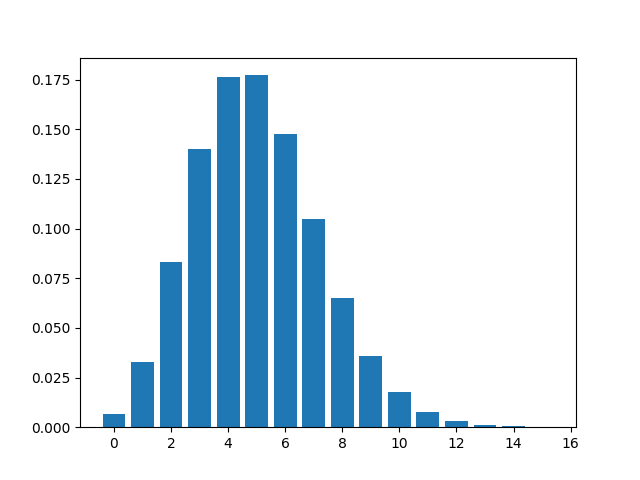
\includegraphics{pic6.png}
\end{center}


\begin{center}
	{\LARGE
		\textbf{فصل سوم}
	}
\end{center}

\textbf{جواب سوال اول:}\\

		\fontsize{11}{11}\selectfont
\begin{latin}
	\begin{lstlisting}
		
def calculate_expected_value(p1,p2,x1,x2):
  return (p1 * x1) + (p2 * x2)

def solving_chapter2_problem_c3_q1():
  py_1 = 1/3
  py_2 = 1 - py_1

  gx_1 = 1
  gx_2 = 2

  print('Showing PMF:')
  print(f'--py(1) = P(X <= 1/3) = {py_1}')
  print(f'--py(2) = P(X <= 1/3) = {py_2}')

  print('-' * 60)

  expected_value = calculate_expected_value(py_1,py_2,gx_1,gx_2)
  print('Showing expected value')
  print(f'--E[Y] = (1/3 * 1) + (2/3 * 2) = {expected_value}')
		
		
	\end{lstlisting}
\end{latin}
\fontsize{14}{14}\selectfont


احتمال مقدار gx در سوال داده شده است. همچنین مقدار آنها 1 و 2 میباشند. در ابتدا PMF این مقادیر را رسم میکنیم و بعد از آن مقدار value expected یا مقدار مورد انتظار را بدست می آوریم. برای بدست آوردن value expected این مقادیر، از تابع calculate\_expected\_value استفاده میکنیم و سپس آن را نمایش میدهیم.\\

خروجی این کد به صورت زیر است:\\


\begin{latin}
	\begin{lstlisting}
		
Showing PMF:
--py(1) = P(X <= 1/3) = 0.3333333333333333
--py(2) = P(X <= 1/3) = 0.6666666666666667
---------------------------------------------------
Showing expected value
--E[Y] = (1/3 * 1) + (2/3 * 2) = 1.6666666666666667
		
	\end{lstlisting}
\end{latin}

\textbf{جواب سوال پنجم}\\


		\fontsize{11}{11}\selectfont
\begin{latin}
	\begin{lstlisting}
		
def solving_chapter2_problem_c3_q5():
  h = 10 #
  x = np.random.uniform(0,h, 1000)
  x_s = sort(x)

  pdf =[ 2*(h - t) / h**2 for t in x_s]

  plt.xlabel('x')
  plt.ylabel('$f_{X}(x)$')
  plt.title('PDF')
  plt.bar(x_s, pdf)
  plt.show()

  plt.rcParams["figure.autolayout"] = True
  cdf = cumsum(pdf)
  plt.plot(x_s, cdf, label="CDF")
  plt.legend()
  plt.show()

  cdf =[1-((h-t)/h)**2 for t in x_s]
  plt.xlabel('x')
  plt.ylabel('$F_{X}(x)$')
  plt.title('CDF')
  plt.plot(x_s, cdf, marker='o')
  plt.show()
		
		
	\end{lstlisting}
\end{latin}
\fontsize{14}{14}\selectfont


\lr{h} ارتفاع  و \lr{x} متغیر تصادفی است. نخست \lr{pdf} را محاسبه کرده ایم و سپس \lr{cdf} را به دو روش محاسبه نموده ایم.
ابتدا بوسیله \lr{pdf} و دوم به وسیله فرمول \lr{cdf}.\\

خروجی کار به صورت زیر است:\\

\begin{center}
	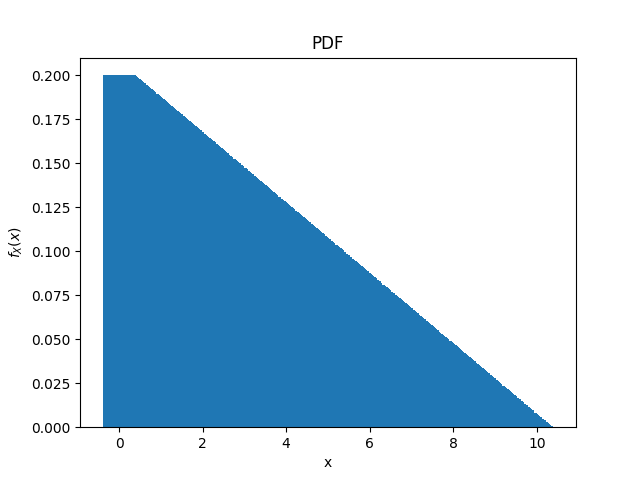
\includegraphics[width=0.8\textwidth]{pic7.png}
\end{center}

\begin{center}
	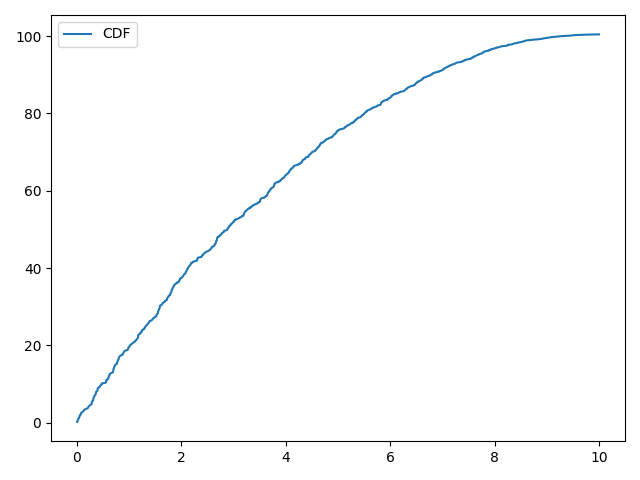
\includegraphics[width=0.8\textwidth]{pic8.png}
\end{center}

\begin{center}
	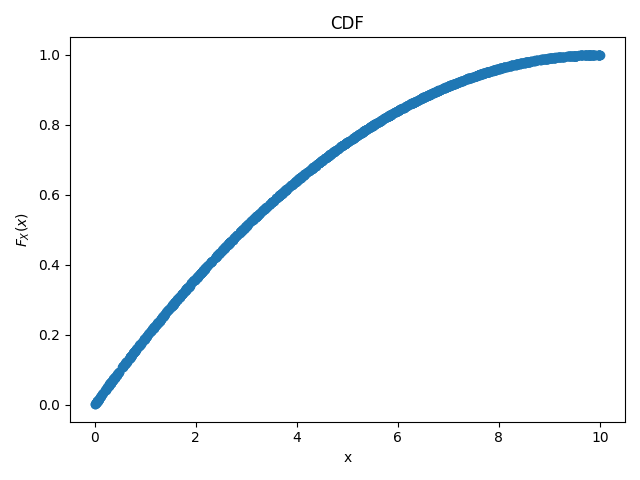
\includegraphics[width=0.8\textwidth]{pic9.png}
\end{center}

\textbf{جواب سوال سیزدهم:}\\


		\fontsize{11}{11}\selectfont
\begin{latin}
	\begin{lstlisting}
		
def normalProbabilityDensity(x):
  constant = 1.0 / np.sqrt(2*np.pi)
  return(constant * np.exp((-x**2) / 2.0))

def solving_chapter2_problem_c3_q13():
  Fahrenheit = 59
  mean = 10
  e = 10
  Celsius = (Fahrenheit - 32) * 5.0/9.0
  z_upper = (Celsius - e)/mean
  temperature, _ = quad(normalProbabilityDensity, np.NINF, z_upper)
  print('Probability: ', temperature)
	\end{lstlisting}
\end{latin}
\fontsize{14}{14}\selectfont




نخست در کد فارنهایت رو به سلسیوس تبدیل کرده ایم که می شود ۱۵ درجه، بعد مقدار z رو محاسبه نموده ایم که از رابطه $(15 -10)/10 = 0.5$ بدست می آید.
سپس بایستی این مقدار را از جدول بررسی کنیم که در پایتون با دستور زیر محاسبه می گردد.

$quad(normalProbabilityDensity, np.NINF, z_upper)$\\

خروجی این کد به صورت زیر است:\\

\begin{latin}
	\begin{lstlisting}
		
Probability:  0.6914624612740132

	\end{lstlisting}
\end{latin}


\textbf{جواب سوال بیست و یکم:}\\

\fontsize{11}{11}\selectfont
\begin{latin}
	\begin{lstlisting}
def solving_chapter2_problem_c3_q21():
  l = input("Please enter length l: ")
  l = int(l)
  x = [0 , l]
  y = [(1/l) , (1/l)]
  plt.plot(x, y)
  plt.xlabel('Y')
  plt.ylabel('Probability')
  plt.title('Probability function of Y')
  plt.show()
  y_in = input("Please enter length of first cut: ")
  y_in = int(y_in)


  x1 = [0, l]
  y1 = [(1 / l), (1 / l)]
  # plotting the line 1 points
  plt.plot(x1, y1, label="Probability function of Y")

  # line 2 points
  x2 = [0, y_in]
  y2 = [(1 / y_in), (1 / y_in)]
  # plotting the line 2 points
  plt.plot(x2, y2, label="Probability function of X|Y")

  # naming the x axis
  plt.xlabel('Probability')
  # naming the y axis
  plt.ylabel('')
  # giving a title to my graph
  plt.title('Probability function of Y and X|Y')

  # show a legend on the plot
  plt.legend()

  # function to show the plot
  plt.show()

  input("Please enter any key to calculate joint PDF of Y and X ")
  x = [0, y_in]
  y = [(1 / l)*(1 / y_in) , (1 / l)*(1 / y_in)]
  plt.plot(x, y)
  plt.xlabel('X,Y')
  plt.ylabel('Probability')
  plt.title('Joint probability function of X,Y')
  plt.show()
  print('-------------------------------------')
  print()
  print('The marginal PDF of X is: 1/l ln(l/x)')
  print('E[X] = l/4')
	\end{lstlisting}
\end{latin}
\fontsize{14}{14}\selectfont


خروجی این کد بستگی به مقدار پارامتر ورودی دارد. در زیر بر اساس مقدار l برابر 4 و اولین برش برابر 2 نتایج آورده شده است:\\


\begin{latin}
	\begin{lstlisting}
Please enter length l: 4
Please enter length of first cut: 2
Please enter any key to calculate joint PDF of Y and X 
----------------------------------------------------

The marginal PDF of X is: 1/l ln(l/x)
E[X] = l/4
	\end{lstlisting}
\end{latin}

\begin{center}
	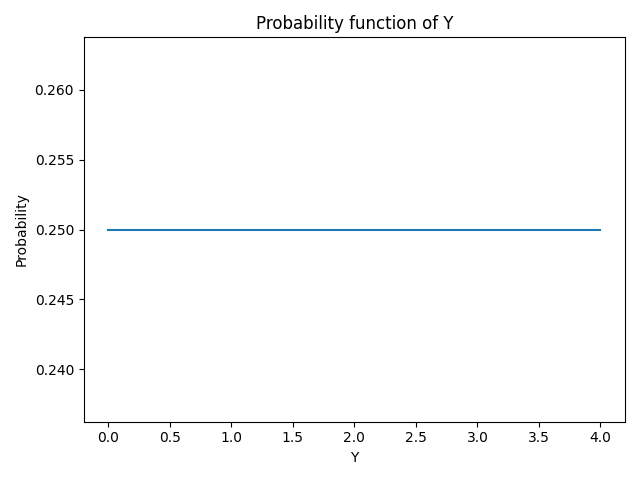
\includegraphics[width=0.8\textwidth]{pic10.png}
\end{center}

\begin{center}
	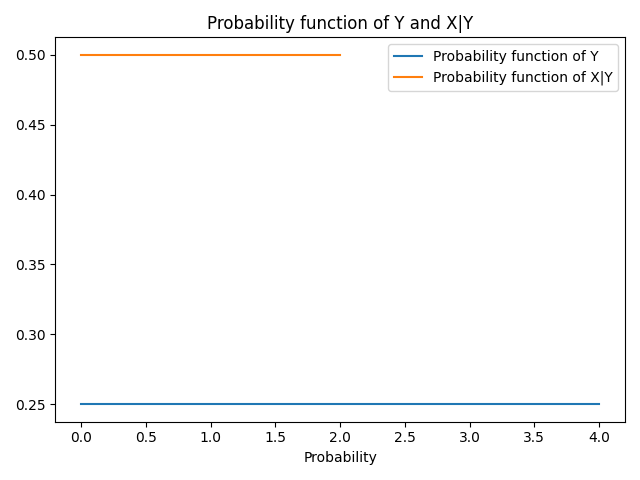
\includegraphics[width=0.8\textwidth]{pic11.png}
\end{center}

\begin{center}
	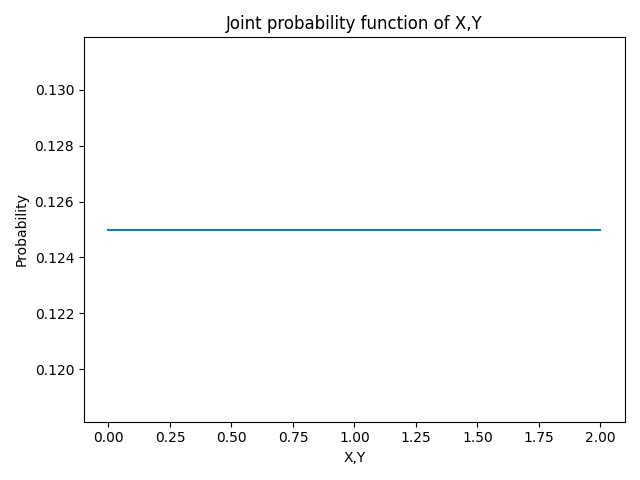
\includegraphics[width=0.8\textwidth]{pic12.png}
\end{center}


\textbf{جواب سوال بیست و پنجم:}\\


\fontsize{11}{11}\selectfont
\begin{latin}
	\begin{lstlisting}

def solving_chapter2_problem_c3_q25():
  sigma = input("Please enter σ value: ")
  sigma = float(sigma)
  c = np.arange(-10, 5, 0.01)
  y = np.exp(-((pow(c,2))/(2*pow(sigma,2))))
  print('Values of c: ', c)
  print('Values of P(c): ', y)

  plt.plot(c, y)

  plt.title("Probability of C^2 <= X^2 + Y^2")
  plt.xlabel("Values of c")
  plt.ylabel("Values of P(c)")
  plt.show()

	\end{lstlisting}
\end{latin}
\fontsize{14}{14}\selectfont

در این سوال پس از اجرای کد مقدار سیگما از کاربر اخذ می شود و دریافت این مقدار نمودار آن رسم می گردد.\\

جواب این سوال با توجه به مقدار ورودی فرق میکند. در زیر خروجی به ازای مقدار ورودی 5 آمده است:\\
\fontsize{11}{11}\selectfont
\begin{latin}
	\begin{lstlisting}

Please enter σ value: 5
Values of c:  [-10.    -9.99  -9.98 ...   4.97   4.98   4.99]
Values of P(c):  [0.13533528 0.13587744 0.13642122 
  ... 0.6101698  0.60895677 0.60774372]

	\end{lstlisting}
\end{latin}
\fontsize{14}{14}\selectfont

\begin{center}
	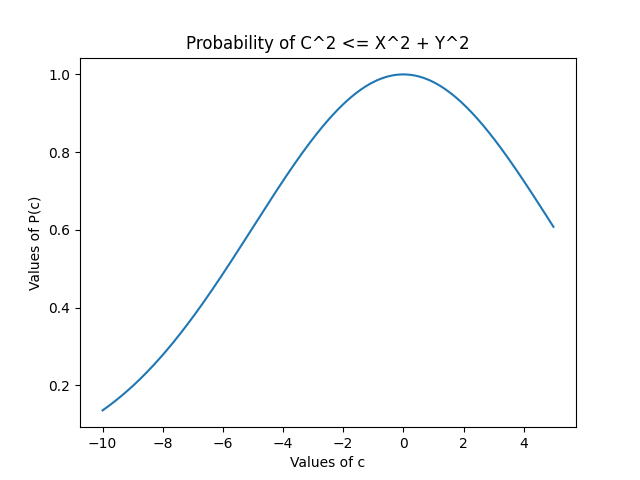
\includegraphics[width=0.8\textwidth]{pic13.png}
\end{center}


\end{document}














